\section{Observations}

\subsection{Observations Task 1}
\todo{what information could be retrieved from the implemented technique?}
\todo{was the task accomplished?}
\todo{pros, cons, improvements}

task 1a
- taking some general attributes such as those in $S_{attr}$ mainly show rather obvious relations:
    > AANTAL_INW == AANTAL_HH
    > OPP_TOT inverse BEV_DICHTH
    > STED inverse OAD
- quite some attributes with a few outliers that mess up the scale of the axis
OPP_TOT, OAD, AANTAL_INW, AANTAL_HH
    this makes it harder to detect relations between the attributes of the more general municipalities, because they lie very close to each other on the axis.


task 1b
- again because the scaling, it also becomes harder to compare municipalities 
OPP_TOT, OAD, AANTAL_HH,
-> con: outliers rack up the scaling -> solution: scale the axes to selection
- student cities have highest percentage of single households (P_EENP_HH)
- municipalicites with low STED value fluctuate more on the other attributes

\begin{figure}[h!]
    \centering
    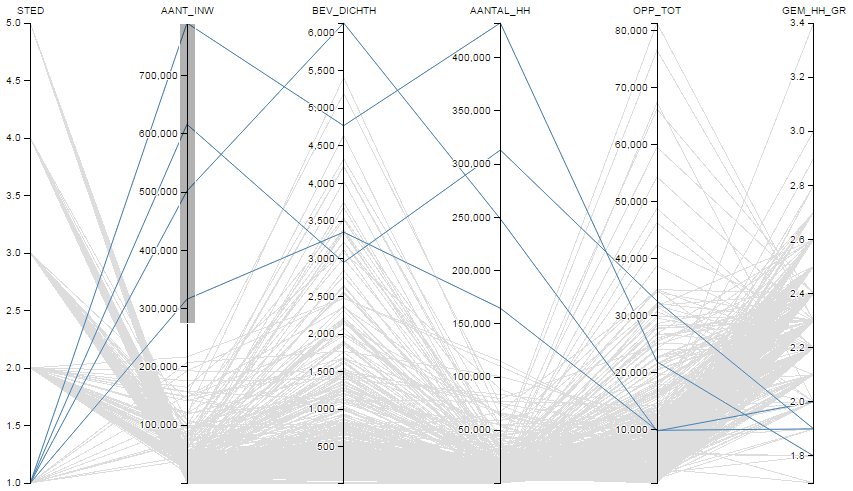
\includegraphics[width=0.8\textwidth]{img/para_outliers.png}
    \caption{Outliers in the Parallel Coordinate Plot}
    \label{fig:para_outliers}
\end{figure}

\subsection{Observations Task 2}
\todo{what information could be retrieved from the implemented technique?}
\todo{was the task accomplished?}
\todo{pros, cons, improvements}

